\subsubsection{Immix}
Implementare in modo ingenuo un algoritmo mark-region è molto facile: la memoria è divisa in zone di dimensione fissata, che possono essere libere o allocate. Durante l'allocazione vengono riempite le regioni disponibili fino a quando la memoria non è esaurita. A quel punto parte la collection. Vengono quindi marcate tutte le regioni con oggetti attivi come non disponibili, e tutte le altre come libere. Gli oggetti, inoltre, non possono estendersi su più regioni. 

Un approccio di questo tipo evidenzia due problemi. Il primo riguarda il dimensionamento delle regioni. Il secondo riguarda la deframmentazione: una regione è non disponibile fintanto che contiene un oggetto vivo, quindi è necessario deframmentare per recuperare più memoria.

Immix risolve il problema operando a due livelli: \textbf{blocchi} e \textbf{linee}. Quando, durante l'allocazione, viene riciclato un blocco, la procedura salta le linee occupate e alloca solo linee libere contigue. Gli oggetti possono occupare più linee, ma non più blocchi. Quando è necessario deframmentare viene eseguita una procedura di evacuazione.

\paragraph{Algoritmo migliorato} 
\subparagraph{Allocazione iniziale.} Inizialmente tutti i blocchi sono liberi. Un allocatore locale al thread ottiene un blocco libero dall'allocatore globale e lo usa per salvare gli oggetti. Se esaurisce il blocco ne chiede un altro, fino a quando lo heap non è esaurito.
\subparagraph{Identificazione.} Tutti gli oggetti vivi vengono tracciati a partire dalla radice dell'applicazione. Anche le corrispondenti linee vengono marcate.
\subparagraph{Pulizia.} Quando l'identificazione è completata, Immix analizza la mappa delle linee per identificare sia i blocchi liberi che le linee libere (in blocchi parzialmente liberi) e ritorna i primi ad una riserva globale e ricicla le seconde per le successive allocazioni.
\subparagraph{Successive allocazioni.} Il thread ricomincia la procedura di allocazione a partire di blocchi riciclati, saltando i blocchi completamente pieni o vuoti e seguendo l'ordine degli indirizzi. Quando viene trovato un buco (delle linee libere contigue, anche una sola), l'oggetto viene salvato (anche parzialmente). Se il buco viene esaurito si prosegue, fino ad esaurire i blocchi riciclati. A quel punto si passa a quelli completamente vuoti, fino ad esaurimento.

Figura~\ref{fig:immixheap} mostra un esempio.
\begin{figure}[h]
	\centering
	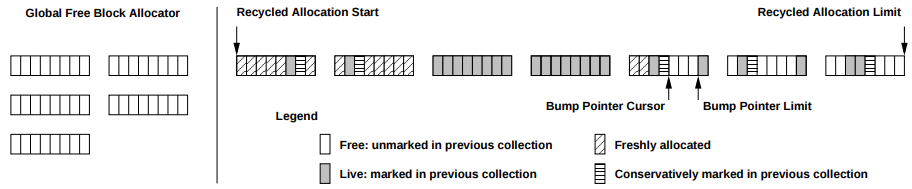
\includegraphics[width=1.2\linewidth]{images/immixHeap}
	\caption[Organizzazione dello heap]{Organizzazione dello heap in Immix}
	\label{fig:immixheap}
\end{figure}

\paragraph{Scelte implementative} 
\subparagraph{Politica di ''riciclaggio''.} Alla fine della pulizia ogni blocco è in uno e solo uno dei seguenti stati: libero, occupato o riciclabile. L'algoritmo marca come riciclabili quei blocchi con almeno \textbf{F} linee libere. Simulazioni hanno portato a scegliere F = 1.
\subparagraph{Politica di allocazione.} Immix alloca seguendo l'ordine degli indirizzi. Esistono altri ordinamenti per cercare di massimizzare la verosimiglianza di trovare blocchi liberi, ma i test hanno mostrato che quello scelto (che è molto semplice) è migliore. 
\subparagraph{Parallelismo.} L'implementazione è parallela e supporta più thread sia lato GC che lato applicazione. Tuttavia la pulizia non viene fatta concorrentemente all'esecuzione dell'applicazione. L'analisi dei blocchi è fatta in parallelo e permette race conditions nella marcatura degli oggetti (al più un oggetto verrà marcato più volte). Per evitare race conditions nell'aggiornamento di bit vicini vengono utilizzato interi byte per marcare le linee. Questo causa un overhead di 1/128, ma evita il bisogno di sincronizzazione. Questo approccio si comporta bene per thread veloci e non sincronizzati (sincronizzando solo i thread del GC) su sistemi monoprocessore o con due core. 
\subparagraph{Overflow Allocation on demand.} Allocare oggetti medi (più grandi di una linea) in blocchi frammentati può portare a sprecare grandi quantità di spazio. Per questo è utile utilizzare un \textit{overflow allocator}. Se Immix non riesce a soddisfare una richiesta rispetto allo spazio disponibile nel blocco corrente, ma ci sono blocchi totalmente liberi, l'oggetto viene allocato in uno di questi per evitare di sprecare spazio (e così l'oggetto è contiguo). Dato che spesso gli oggetti Java sono piccoli e che una linea può ospitare più oggetti, questa ottimizzazione permette di usare lo spazio in modo più efficiente.

\paragraph{Deframmentazione} \mbox{} \\
Un algoritmo mark-region non-moving è naturalmente soggetto a frammentazione. Sia l'evacuazione che il compattamento sono soluzioni ben conosciute, ma Immix utilizza un approccio più opportunistico. All'inizio di ogni pulizia determina se deframmentare o no a seconda del livello di frammentazione rilevato nelle precedenti analisi. 

Quando viene trovato un oggetto attivo in un blocco candidato, questo viene valutato. Viene evacuato solo se l'applicazione non l'ha bloccato e se lo spazio riservato per l'evacuazione non è terminato. Se un oggetto è inamovibile viene marcato come vivo e lasciato su quella locazione. Altrimenti, viene evacuato e sostituito con un puntatore alla nuova posizione. Se vengono trovati altri riferimenti dello stesso oggetto, questi vengono rimpiazzati con quel puntatore. Immix riserva un piccolo numero di blocchi completamente liberi come area per l'evacuazione: in generale lo spazio corrisponde al 2.5\%, ma può essere alzato a 3\% in condizioni di utilizzo intensivo.

\subparagraph{Selezione dei candidati.} Un sacco di euristiche possono essere utilizzate per selezionare i candidati alla deframmentazione. La strategia utilizzata è di tipo on demand. Se ci sono uno o più blocchi riciclabili non utilizzati dall'allocatore o se la precedente pulizia non ha liberato abbastanza spazio, Immix programma la deframmentazione per la prossima collezione. A questo punto vengono selezionati i blocchi con più buchi. Usa anche i dati raccolti nell'ultima analisi per selezionare quanti più blocchi possibili. Per calcolare queste stime velocemente vengono utilizzati due istogrammi basati sul conteggio dei buchi. Uno stima lo spazio richiesto (\textit{mark histogram}) e l'altro riflette lo spazio disponibile (\textit{available histogram}). Il primo è costruito in modo eager durante la pulizia alla fine di ciascuna collezione. Immiz marca ogni blocco con il numero dei suoi buchi e aggiorna l'istogramma per indicare la distribuzione delle linee marcate nello heap in funzione del numero di buchi associati al blocco. Queste operazioni sono economiche e possono essere fatte alla fine di ogni collezione, anche se non sarà effettuata deframmentazione. Il secondo, invece, viene creato in modo lazy, solamente quando si decide di deframmentare. Ogni barra dell'istogramma riflette il numero di linee disponibili all'interno del blocco. Per identificare i candidati, Immix percorre l'istogramma, partendo dal punto di maggiore frammentazione. Incrementa lo spazio richiesto per il volume nella corrispondente barra del mark histogram e lo decrementa per il volume della barra dell'available histogram. Quando incontra un blocco per il quale la stima eccede il reale spazio disponibile, candida tutti i blocchi incontrati precedentemente per la deframmentazione. 

\subparagraph{Deframmentazione parallela.} Durante la deframmentazione è necessario sincronizzarsi per evitare che un oggetto venga evacuato in due posizioni per una race condition. 

\subparagraph{Pinning.} In alcune situazioni un'applicazione può chiedere che un oggetto non venga mosso. Sebbene questa funzionalità non sia direttamente supportata in Java, alcune implementazioni della VM possono richiederlo (ad esempio per migliorare la gestione del buffer per l'I/O da file). Di conseguenza Immix supporta direttamente questa possibilità, e non sposta gli oggetti per i quali l'applicazione fa pinning.

\paragraph{Valutazione} \mbox{} \\
Questa sezione analizza le prestazioni di Immix rispetto ad altri tre algoritmi di tre strategie diverse: \textbf{mark-sweep} (‘MS’, sweep-to-free-list), \textbf{semi-space} (‘SS’, evacuate),
e \textbf{mark-compact} (‘MC’, compact). 

Figura~\ref{fig:heapallocation} mostra l'efficienza in termini di spazio. Si nota che Immix si comporta generalmente meglio rispetto agli altri, tanto da essere sempre tra i migliori in termini di gestione delle allocazioni sullo heap. Come prevedibile SS, che occupa generalmente il doppio dello spazio a causa dell'evacuazione, è il peggiore. Immix si comporta generalmente meglio di MS, grazie alla gestione della memoria utilizzando due diverse granularità, ed ha un comportamento simile (e a volte addirittura migliore), di MC. Questo significa che la strategia di allocazione di Immix e tutte le ottimizzazioni inserite (gestione degli overflow e riciclaggio dei blocchi parzialmente occupati) consente di gestire lo spazio in modo migliore. Infatti, reclamare memoria a livello di linea consente di operare ad una granularità molto fine, sfruttando l'osservazione empirica che molto spesso gli oggetti Java sono di piccole dimensioni.
\begin{figure}[h]
	\centering
	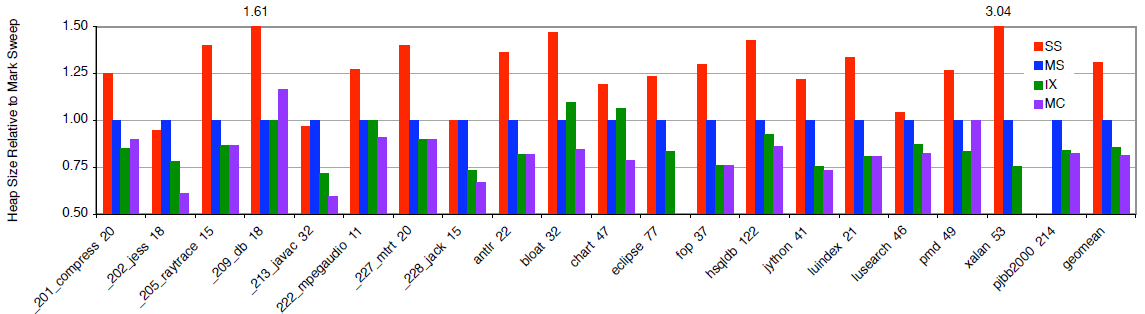
\includegraphics[width=0.7\linewidth]{heapAllocation}
	\caption[Efficienza di spazio]{Efficienza di spazio per vari algoritmi RTGC}
	\label{fig:heapallocation}
\end{figure}

Figura~\ref{fig:rtgc} mostra invece un confronto basato sulle performance dell'applicazione (Figura~\ref{fig:mutuatorPerformance}) e del processo di pulizia. (Figura~\ref{fig:fastCollection}). Come prevedibile la prima indica che le strategie SS e MC consentono all'applicazione prestazioni molto alte. Il motivo è, naturalmente, che queste due strategie allocano gli oggetti in maniera contigua, e di conseguenza l'applicazione ha tempi di esecuzione minori. AL contrario MS si comporta molto male, perché la sua politica causa molta frammentazione nella memoria. Immix si posiziona molto più in basso (e quindi ha un risultato molto migliore) di MS, arrivando quasi agli stessi livelli di SS e MC. Questo grazie alla deframmentazione opportunistica che viene eseguita on-demand solo quando è necessario. L'esecuzione on-demand consente ad Immix di non incorrere in un peggioramento di performance significativo durante la pulizia, come si può notare in Figura~\ref{fig:fastCollection}. Il tempo di collezione è praticamente uguale a quello di MS. Il risultato è coerente dato che il principio di base è lo stesso, l'unica variazione è la granularità a cui Immix opera. Al contrario MC e SS richiedono molto più tempo, come prevedibile dato che mantengono la memoria contigua ad ogni pulizia, e quindi incorrono in un overhead significativo.
\begin{figure}
	\centering
	\begin{subfigure}[b]{0.4\textwidth}
		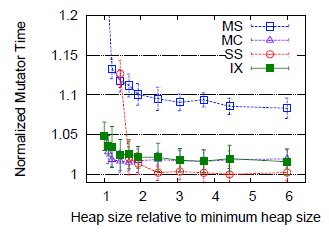
\includegraphics[width=\textwidth]{mutuatorPerformance}
		\caption{Performance dell'applicazione sotto GC}
		\label{fig:mutuatorPerformance}
	\end{subfigure}
	~
	\begin{subfigure}[b]{0.4\textwidth}
		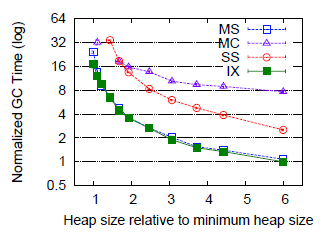
\includegraphics[width=\textwidth]{fastCollection}
		\caption{Tempo richiesto per la pulizia}
		\label{fig:fastCollection}
	\end{subfigure}
	\caption[Confronto di algoritmi RTCG]{Confronto di algoritmi RTCG basato sulle performance dell'applicazione e sul tempo di pulizia}\label{fig:rtgc}
\end{figure}

In definitiva, quindi, Immix raggiunge tutti e tre gli obiettivi necessari ad essere un buon algoritmo di RTGC: efficienza di allocazione (Figura~\ref{fig:heapallocation}), processo di collezione veloce (Figura~\ref{fig:fastCollection}) e non degrado delle performance dell'applicazione (Figura~\ref{fig:mutuatorPerformance}).